\chapter{Initial proposal}\label{C:innitial-proposal}
This project was proposed by AlterAid a company which is working on several ways to help in taking care of the health of our elderly, or in general, anyone that is relevant to our lives.

This company is working on two different projects that combine together, the first one is called aaaida which consists of a social network where people can stay alert about its relatives, upload information about its health or watch recommendations from doctors. On the other side, and more hardware oriented development, they are creating a Sensor Network called HomeSense that once deployed in a house will be able to collect relevant information from those sensors in the home and allow other people to know if the daily life is going normal, or something is happening.


\section{AlterAid products in depth}\label{S:alteraid-products}
As explained before, AlterAid has two relevant products, aaaida which is the unifying social network that shows or even analyzes
the data uploaded there. Then comes HomeSense, a Wireles Healthcare Sensor Platform, which is interesting on terms of sensing and daily life control. HomeSense idea is be capable of pick information using distributed sensors around a house and then upload to aaaida.

\subsection{Aaaida}\label{SS:Aaaida-proposal}


\subsection{HomeSense}\label{SS:HomeSense-proposal}


\subsection{Case of use}\label{SS:Case-Of-Use}
Alice is a young teenager whose grandfather, Bob, is ill and she wants to know if all is fine in Bob's home life. Alice will sign up in http://www.aaaida.com, there she will create a bond called Bob. A bond is a entity that represents a person, this entity can be configured with different measures. Then Alice will create 2 measures, the first one will be blood pressure while the other one will be bob's house.
In blood pressure, Bob will use a simple elderly-oriented mobile application in order to upload his blood pressure every day, in this manner Alice can be aware of its health.
Apart from this, Alice will buy a product from AlterAid, called HomeSense, which consists of a set of sensors that must be installed in doors, walls, drawers..., a small centralized system that must be plugged to the power and an application to configure HomeSense.
This application will facilitate the linking between Alice account and Bob's bond, in addition, Alice will be able to setup a internet link to HomeSense using grandfather's Internet or a GSM connection to some mobile phone provider.
Once the system is configured and working, Alice will be able to take care of Bob's home life, for example if he must take a pill at the morning, she can control at least if the medicine cabinet has been opened. Or if all doors are closed if Bob is out of home.

\begin{figure}[H]\begin{center}
 \centering
  \captionsetup{justification=centering}
  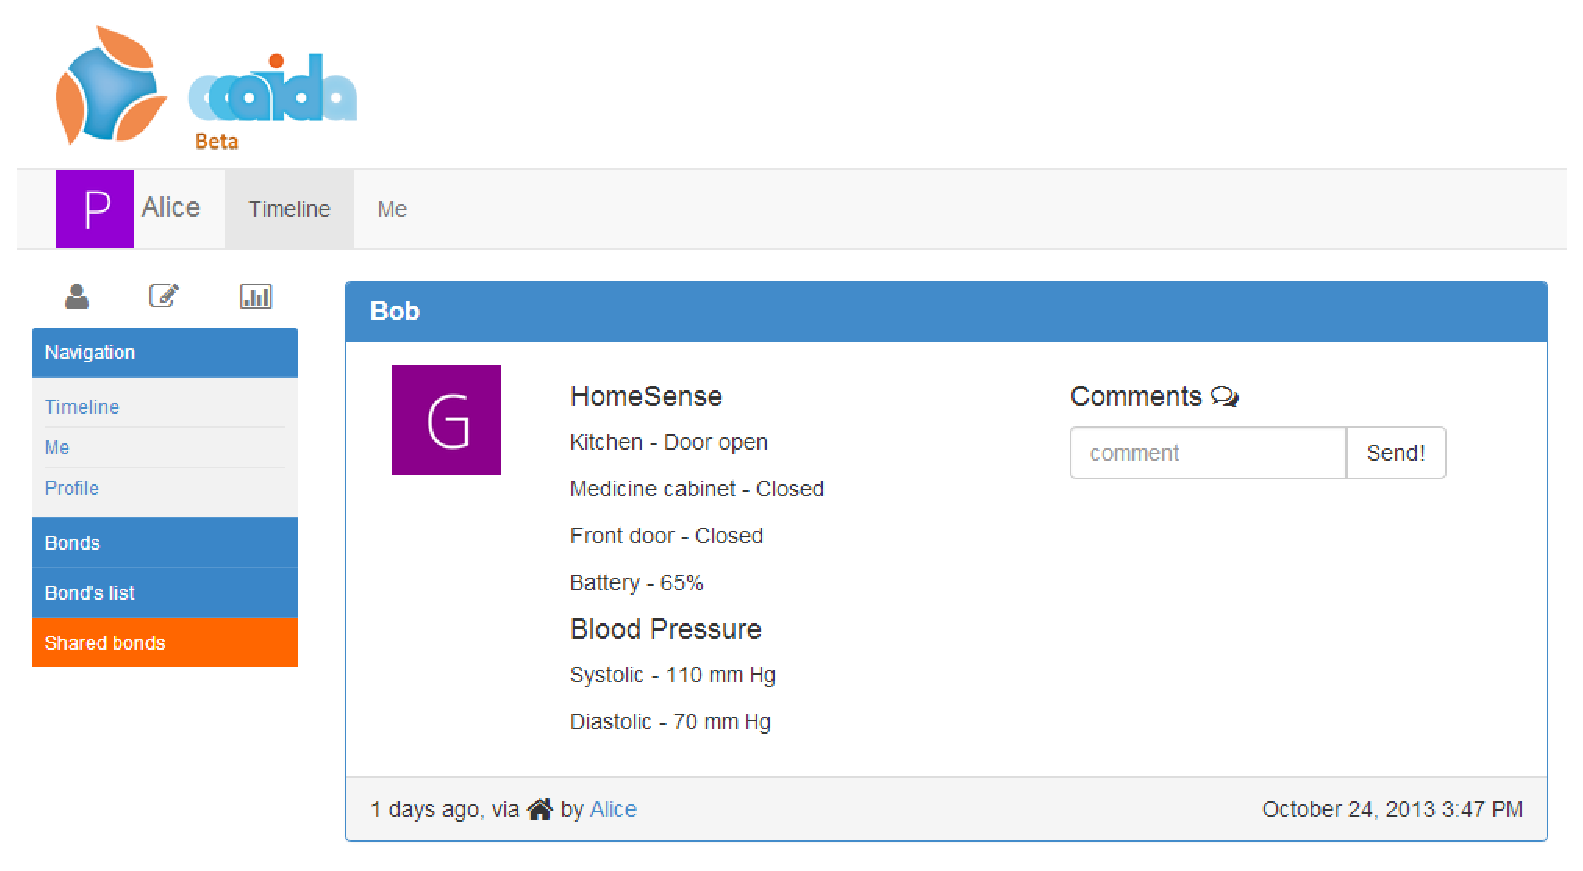
\includegraphics[width=1\textwidth]{pictures/proposal/aaaida-use-case}
  \caption{Case of use representation in aaaida \label{fig:network-architecture}}
\end{center}\end{figure}
%width=\textwidth
%\subsection{Aaaida skeleton}\label{SS:Aaaida-Skeleton}
%Actually aaaida is being developed using Grails, which is a framework that uses Groovy on top of the Java Virtual Machine.
%Grails is a Model-View-Controller(MVC) framework, a MVC pattern in this case fits pretty well:
%\begin{itemize}
%\item{\textbf{Model:} Entities corresponding to Users, Bonds, Measures, Values, Advertisements and Applications.}
%\item{\textbf{View:} Basically is the website interface where people can see advertisments (new data) and configure bonds and measures.}
%\item{\textbf{Controller:} Is the logic of aaaida, it connects to the graph database, processes data and route requests to the endpoints that render views.}
%\end{itemize}

%Apart from this, and in terms of this thesis more relevant, aaaida has an open API working with the RFC6749 (OAuth 2.0).

%\subsection{HomeSense skeleton}\label{SS:HomeSense-Skeleton}
%HomeSense

\section{AlterNative}\label{S:AlterNative}
blablabla AlterNative

\section{Thesis Proposal}\label{S:Thesis-Proposal}
